\begin{frame}{Which decision boundary?}
\begin{columns}
  \begin{column}{0.5\textwidth}
    \begin{itemize}
      \item Multiple decision boundaries can perfectly separate the data.
      \item Which one should we choose?
      \item Some boundaries may generalize better than others.
    \end{itemize}
  \end{column}
  \begin{column}{0.5\textwidth}
    \centering
    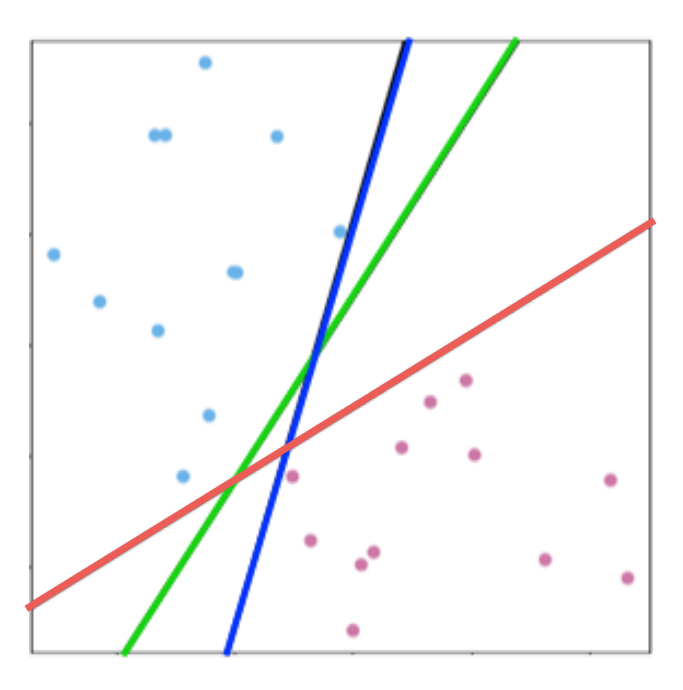
\includegraphics[width=\linewidth]{images/support-vector-machines/support-vector-machines-7.png}
  \end{column}
\end{columns}
\end{frame}

\begin{frame}{Maximal Margin Hyperplane}
\begin{columns}
  \begin{column}{0.5\textwidth}
    \begin{itemize}
      \item Which of the infinite separating hyperplanes should we choose?
      \item A natural choice is the \textbf{maximal margin hyperplane}.
      \item It is the separating hyperplane that is farthest from the training samples.
    \end{itemize}
  \end{column}
  \begin{column}{0.5\textwidth}
    \centering
    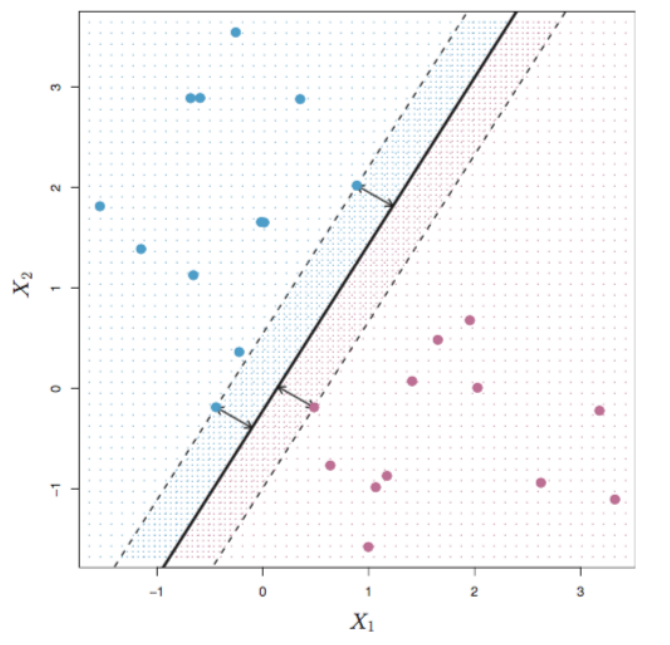
\includegraphics[width=\linewidth]{images/support-vector-machines/support-vector-machines-8.png}
  \end{column}
\end{columns}
\end{frame}


\begin{frame}{Maximal Margin Hyperplane}
\begin{columns}
  \begin{column}{0.5\textwidth}
    \begin{itemize}
      \item Margin: smallest distance between any training observation and the hyperplane.
      \item Support vectors: training observations whose distance to the hyperplane is equal to the margin
    \end{itemize}
  \end{column}
  \begin{column}{0.5\textwidth}
    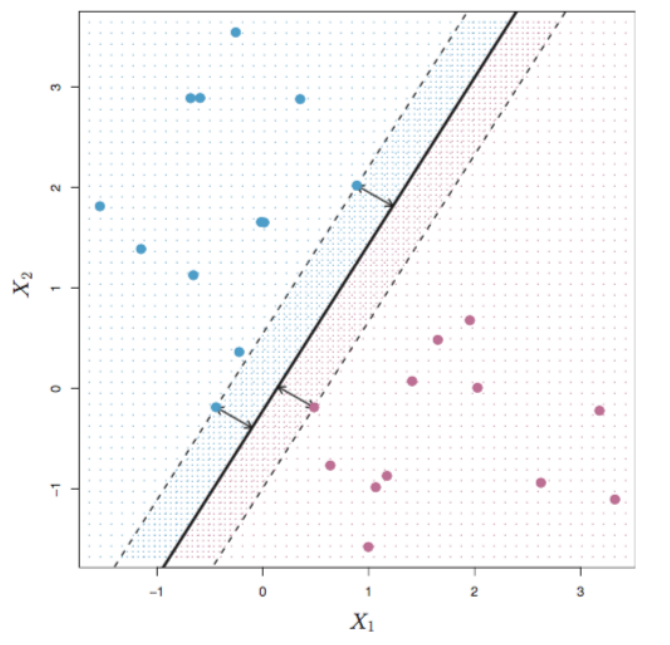
\includegraphics[width=\linewidth]{images/support-vector-machines/support-vector-machines-8.png}
  \end{column}
\end{columns}
\end{frame}


\begin{frame}{Why is it called a support vector?}
\begin{itemize}
  \item “Support”: maximal margin hyperplane only depends on these observations.
  \item “Vector”: points are vectors in $p$-dimensional space.
  \item If support vectors are perturbed, then MM hyperplane will change.
  \item If other training observations perturbed (provided not perturbed within margin distance of hyperplane), then MM hyperplane not affected.
\end{itemize}
\end{frame}


\begin{frame}{Finding Maximal Margin Classifier}
\begin{itemize}
  \item To find the maximal margin hyperplane on data $(\vec{x}^{(i)}, y^{(i)})$, where $y^{(i)} \in \{-1, 1\}$, solve:
\end{itemize}

\[
\max_{\beta_0, \ldots, \beta_p} M
\]

\begin{itemize}
  \item maximize the margin, $M$
\end{itemize}

\[
\text{subject to} \quad \sum_{j=0}^{p} \beta_j^2 = 1
\]

\begin{itemize}
  \item constraint necessary for well-defined optimization problem
\end{itemize}

\[
y^{(i)}\left( \beta_0 + \beta_1 x_1^{(i)} + \ldots + \beta_p x_p^{(i)} \right) \geq M, \quad \forall i
\]

\begin{itemize}
  \item all training points must be at least distance $M$ from hyperplane
\end{itemize}
\end{frame}

\begin{frame}{Finding Maximal Margin Classifier}
\begin{itemize}
  \item To find the maximal margin hyperplane on data $(\vec{x}^{(i)}, y^{(i)})$, where $y^{(i)} \in \{-1, 1\}$, solve:
\end{itemize}
\begin{itemize}
    \item \[ \max_{\beta_0, \ldots, \beta_p} M \]
\end{itemize}

\begin{itemize}
  \item subject to $\sum_{j=0}^{p} \beta_j^2 = 1$
  \item $y^{(i)}\left( \beta_0 + \beta_1 x_1^{(i)} + \ldots + \beta_p x_p^{(i)} \right) \geq M, \quad \forall i$
\end{itemize}

\begin{itemize}
  \item Can be written as a convex optimization problem.
  \item We know how to solve convex optimization problems efficiently to find $M$ and $\beta$.
\end{itemize}
\end{frame}



\begin{frame}{Maximal Margin Classifier}
\begin{columns}
  \begin{column}{0.5\textwidth}
    \begin{itemize}
      \item Recall the assumption: Classes can be separated by a linear decision boundary.
      \item What if there is no separating hyperplane?
    \end{itemize}
  \end{column}
  \begin{column}{0.5\textwidth}
    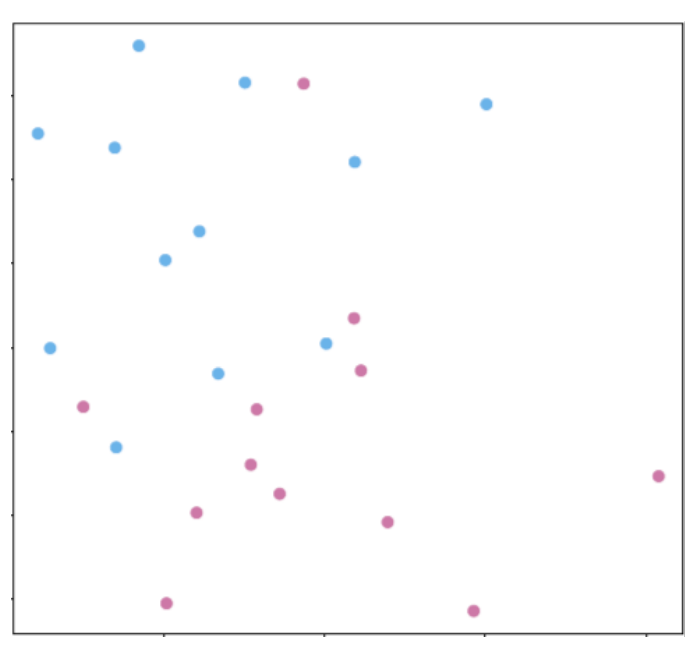
\includegraphics[width=\linewidth]{images/support-vector-machines/support-vector-machines-9.png}
  \end{column}
\end{columns}
\end{frame}


\begin{frame}{Maximal Margin Classifier}
\begin{columns}
  \begin{column}{0.5\textwidth}
    \begin{itemize}
      \item Furthermore, notice a disadvantage of the maximal margin classifier:
      \begin{itemize}
        \item Can be sensitive to individual observations
        \item May overfit training data
      \end{itemize}
    \end{itemize}
  \end{column}
  \begin{column}{0.5\textwidth}
    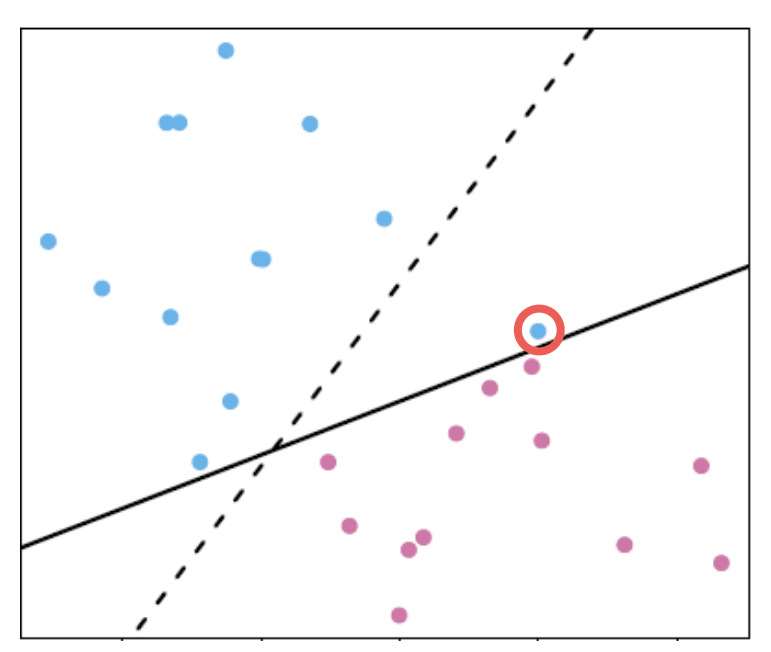
\includegraphics[width=\linewidth]{images/support-vector-machines/support-vector-machines-10.png}
  \end{column}
\end{columns}
\end{frame}
